\section{Tables de la Loi Normale Centrée Réduite.}\label{tablenormale}
\begin{center}
	
	$$\Phi(t)=\prob(X \leq t) = \int_{-\infty}^t\frac{1}{\sqrt{2\pi}}\ e^{-\frac{x^2}{2}}dx\ \ \mbox{ et }\ \ \Phi(-t)=1 - \Phi(t).$$
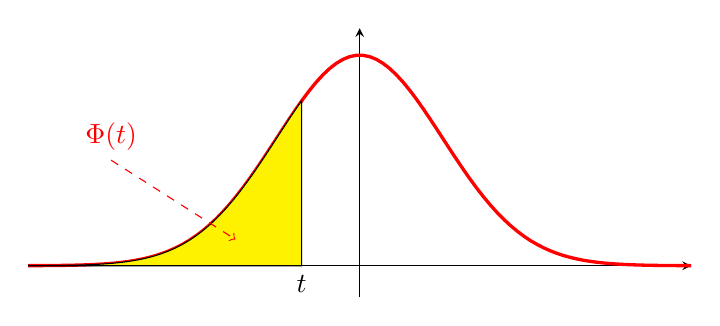
\begin{tikzpicture}
	\def\val{-0.7}
	\def\fval{0.3121}
	
	\begin{axis}[
		axis lines=middle,
		domain=-4:4,
		xtick=\empty,
		ytick=\empty,
		ymin=-0.06, ymax = 0.45,
		enlargelimits=false,
		samples=100,
		width=10cm,
		height=5cm,
		x label style={at={(axis description cs:1.05,0.5)},anchor=north},
		y label style={at={(axis description cs:0.5,1.05)},anchor=west}
		]
		
		\addplot[red, very thick, no markers, domain=-4:4] {exp(-x^2 / (2*1^2)) / (1*sqrt(2*pi))};
		
		\addplot[fill=yellow, domain=-4:\val] {exp(-x^2 / (2*1^2)) / (1*sqrt(2*pi))} \closedcycle;
		
		\draw[dashed, red, ->] (axis cs: -3, 0.2) -- (axis cs: -1.5, 0.05) node[at start, above, red] {$\Phi(t)$};
		
\node[below] at (axis cs: \val, 0) {$t$};
		
	\end{axis}

\end{tikzpicture}


	Voici une table des quantiles les plus couramment utilisées :
	
	\begin{small}
		\begin{center}
			\begin{tabular}{ll}
				\multicolumn{1}{c}{$p$}& \multicolumn{1}{c}{$\Phi^{-1}(p)$} \\ \midrule
				$0.9$ & $1.2815515655$\\
				$0.95$ & $1.6448536270$\\
				$0.975$ & $1.9599639845$\\
				$0.99$ & $2.3263478740$\\
				$0.995$ & $2.5758293035$\\
				$0.9975$ & $2.8070337683$\\
				
				\midrule  
			\end{tabular}
			\hspace*{1.25cm}
			\begin{tabular}{ll}
				\multicolumn{1}{c}{$p$}& \multicolumn{1}{c}{$\Phi^{-1}(p)$} \\ \midrule
				$0.999$ & $3.0902323062$\\
				$0.9995$ & $3.2905267315$\\
				$0.99975$ & $3.4807564043$\\
				$0.9999$ & $3.7190164855$\\
				$0.99995$ & $3.8905918864$\\
				$0.999975$ & $4.0556269811$\\
				
				\midrule  
			\end{tabular}
			\hspace*{1.25cm}
			\begin{tabular}{ll}
				\multicolumn{1}{c}{$p$}& \multicolumn{1}{c}{$\Phi^{-1}(p)$} \\ \midrule
				$0.99999$ & $4.2648907939$\\
				$0.999995$ & $4.4171734135$\\
				$0.9999975$ & $4.5647877303$\\
				$0.999999$ & $4.7534243088$\\
				$0.9999995$ & $4.8916384757$\\
				$0.99999975$ & $5.0263128360$\\
				
				\midrule  
			\end{tabular}
		\end{center}
	\end{small}
\end{center}

La table suivante donne toutes les valeurs de $\Phi(t)$ où $t$ parcourt l'intervalle $[0;3.99]$ par pas de $10^{-2}$.

\begin{center}
\begin{exemple}{}{}
	On lira dans la table ci-contre que $\prob(X \leq 1.96)\approx 97.50\%$.
\end{exemple}

\begin{tabular}{| c | c | c | c | c | c | c | c | c | c | c |}
	\hline
	t & $0.00$ & $0.01$ & $0.02$ & $0.03$ & $0.04$ & $0.05$ & $0.06$ & $0.07$ & $0.08$ & $0.09$  \\
	\hline
	$0.0$ & $0.5000$ & $0.5040$ & $0.5080$ & $0.5120$ & $0.5160$ & $0.5199$ & $0.5239$ & $0.5279$ & $0.5319$ & $0.5359$ \\
	$0.1$ & $0.5398$ & $0.5438$ & $0.5478$ & $0.5517$ & $0.5557$ & $0.5596$ & $0.5636$ & $0.5675$ & $0.5714$ & $0.5753$ \\
	$0.2$ & $0.5793$ & $0.5832$ & $0.5871$ & $0.5910$ & $0.5948$ & $0.5987$ & $0.6026$ & $0.6064$ & $0.6103$ & $0.6141$ \\
	$0.3$ & $0.6179$ & $0.6217$ & $0.6255$ & $0.6293$ & $0.6331$ & $0.6368$ & $0.6406$ & $0.6443$ & $0.6480$ & $0.6517$ \\
	$0.4$ & $0.6554$ & $0.6591$ & $0.6628$ & $0.6664$ & $0.6700$ & $0.6736$ & $0.6772$ & $0.6808$ & $0.6844$ & $0.6879$ \\
	$0.5$ & $0.6915$ & $0.6950$ & $0.6985$ & $0.7019$ & $0.7054$ & $0.7088$ & $0.7123$ & $0.7157$ & $0.7190$ & $0.7224$ \\
	$0.6$ & $0.7257$ & $0.7291$ & $0.7324$ & $0.7357$ & $0.7389$ & $0.7422$ & $0.7454$ & $0.7486$ & $0.7517$ & $0.7549$ \\
	$0.7$ & $0.7580$ & $0.7611$ & $0.7642$ & $0.7673$ & $0.7704$ & $0.7734$ & $0.7764$ & $0.7794$ & $0.7823$ & $0.7852$ \\
	$0.8$ & $0.7881$ & $0.7910$ & $0.7939$ & $0.7967$ & $0.7995$ & $0.8023$ & $0.8051$ & $0.8078$ & $0.8106$ & $0.8133$ \\
	$0.9$ & $0.8159$ & $0.8186$ & $0.8212$ & $0.8238$ & $0.8264$ & $0.8289$ & $0.8315$ & $0.8340$ & $0.8365$ & $0.8389$ \\
	\hline
	$1.0$ & $0.8413$ & $0.8438$ & $0.8461$ & $0.8485$ & $0.8508$ & $0.8531$ & $0.8554$ & $0.8577$ & $0.8599$ & $0.8621$ \\
	$1.1$ & $0.8643$ & $0.8665$ & $0.8686$ & $0.8708$ & $0.8729$ & $0.8749$ & $0.8770$ & $0.8790$ & $0.8810$ & $0.8830$ \\
	$1.2$ & $0.8849$ & $0.8869$ & $0.8888$ & $0.8907$ & $0.8925$ & $0.8944$ & $0.8962$ & $0.8980$ & $0.8997$ & $0.9015$ \\
	$1.3$ & $0.9032$ & $0.9049$ & $0.9066$ & $0.9082$ & $0.9099$ & $0.9115$ & $0.9131$ & $0.9147$ & $0.9162$ & $0.9177$ \\
	$1.4$ & $0.9192$ & $0.9207$ & $0.9222$ & $0.9236$ & $0.9251$ & $0.9265$ & $0.9279$ & $0.9292$ & $0.9306$ & $0.9319$ \\
	$1.5$ & $0.9332$ & $0.9345$ & $0.9357$ & $0.9370$ & $0.9382$ & $0.9394$ & $0.9406$ & $0.9418$ & $0.9429$ & $0.9441$ \\
	$1.6$ & $0.9452$ & $0.9463$ & $0.9474$ & $0.9484$ & $0.9495$ & $0.9505$ & $0.9515$ & $0.9525$ & $0.9535$ & $0.9545$ \\
	$1.7$ & $0.9554$ & $0.9564$ & $0.9573$ & $0.9582$ & $0.9591$ & $0.9599$ & $0.9608$ & $0.9616$ & $0.9625$ & $0.9633$ \\
	$1.8$ & $0.9641$ & $0.9649$ & $0.9656$ & $0.9664$ & $0.9671$ & $0.9678$ & $0.9686$ & $0.9693$ & $0.9699$ & $0.9706$ \\
	$1.9$ & $0.9713$ & $0.9719$ & $0.9726$ & $0.9732$ & $0.9738$ & $0.9744$ & $0.9750$ & $0.9756$ & $0.9761$ & $0.9767$ \\
	\hline
	$2.0$ & $0.9772$ & $0.9778$ & $0.9783$ & $0.9788$ & $0.9793$ & $0.9798$ & $0.9803$ & $0.9808$ & $0.9812$ & $0.9817$ \\
	$2.1$ & $0.9821$ & $0.9826$ & $0.9830$ & $0.9834$ & $0.9838$ & $0.9842$ & $0.9846$ & $0.9850$ & $0.9854$ & $0.9857$ \\
	$2.2$ & $0.9861$ & $0.9864$ & $0.9868$ & $0.9871$ & $0.9875$ & $0.9878$ & $0.9881$ & $0.9884$ & $0.9887$ & $0.9890$ \\
	$2.3$ & $0.9893$ & $0.9896$ & $0.9898$ & $0.9901$ & $0.9904$ & $0.9906$ & $0.9909$ & $0.9911$ & $0.9913$ & $0.9916$ \\
	$2.4$ & $0.9918$ & $0.9920$ & $0.9922$ & $0.9925$ & $0.9927$ & $0.9929$ & $0.9931$ & $0.9932$ & $0.9934$ & $0.9936$ \\
	$2.5$ & $0.9938$ & $0.9940$ & $0.9941$ & $0.9943$ & $0.9945$ & $0.9946$ & $0.9948$ & $0.9949$ & $0.9951$ & $0.9952$ \\
	$2.6$ & $0.9953$ & $0.9955$ & $0.9956$ & $0.9957$ & $0.9959$ & $0.9960$ & $0.9961$ & $0.9962$ & $0.9963$ & $0.9964$ \\
	$2.7$ & $0.9965$ & $0.9966$ & $0.9967$ & $0.9968$ & $0.9969$ & $0.9970$ & $0.9971$ & $0.9972$ & $0.9973$ & $0.9974$ \\
	$2.8$ & $0.9974$ & $0.9975$ & $0.9976$ & $0.9977$ & $0.9977$ & $0.9978$ & $0.9979$ & $0.9979$ & $0.9980$ & $0.9981$ \\
	$2.9$ & $0.9981$ & $0.9982$ & $0.9982$ & $0.9983$ & $0.9984$ & $0.9984$ & $0.9985$ & $0.9985$ & $0.9986$ & $0.9986$ \\
	\hline
	$3.0$ & $0.9987$ & $0.9987$ & $0.9987$ & $0.9988$ & $0.9988$ & $0.9989$ & $0.9989$ & $0.9989$ & $0.9990$ & $0.9990$ \\
	$3.1$ & $0.9990$ & $0.9991$ & $0.9991$ & $0.9991$ & $0.9992$ & $0.9992$ & $0.9992$ & $0.9992$ & $0.9993$ & $0.9993$ \\
	$3.2$ & $0.9993$ & $0.9993$ & $0.9994$ & $0.9994$ & $0.9994$ & $0.9994$ & $0.9994$ & $0.9995$ & $0.9995$ & $0.9995$ \\
	$3.3$ & $0.9995$ & $0.9995$ & $0.9995$ & $0.9996$ & $0.9996$ & $0.9996$ & $0.9996$ & $0.9996$ & $0.9996$ & $0.9997$ \\
	$3.4$ & $0.9997$ & $0.9997$ & $0.9997$ & $0.9997$ & $0.9997$ & $0.9997$ & $0.9997$ & $0.9997$ & $0.9997$ & $0.9998$ \\
	$3.5$ & $0.9998$ & $0.9998$ & $0.9998$ & $0.9998$ & $0.9998$ & $0.9998$ & $0.9998$ & $0.9998$ & $0.9998$ & $0.9998$ \\
	$3.6$ & $0.9998$ & $0.9998$ & $0.9999$ & $0.9999$ & $0.9999$ & $0.9999$ & $0.9999$ & $0.9999$ & $0.9999$ & $0.9999$ \\
	$3.7$ & $0.9999$ & $0.9999$ & $0.9999$ & $0.9999$ & $0.9999$ & $0.9999$ & $0.9999$ & $0.9999$ & $0.9999$ & $0.9999$ \\
	$3.8$ & $0.9999$ & $0.9999$ & $0.9999$ & $0.9999$ & $0.9999$ & $0.9999$ & $0.9999$ & $0.9999$ & $0.9999$ & $0.9999$ \\
	$3.9$ & $1.0000$ & $1.0000$ & $1.0000$ & $1.0000$ & $1.0000$ & $1.0000$ & $1.0000$ & $1.0000$ & $1.0000$ & $1.0000$ \\
	\hline
	\hline
\end{tabular}
\end{center}



\pagebreak

\section{Loi du $\chi^2$}
$$F_{\nu}(t)=\prob(X \leq t)$$

La table suivante contient les quantiles de la loi $\chi^2$ avec $\nu$ degrés de liberté. Pour tout $0<p<1$, le quantile est la valeur de $t$ pour laquelle $\prob\{X\leq t\}=p$, où $X\sim \chi^2(\nu)$. Ainsi $t=F^{-1}_{\nu}(p)$.

%\begin{center}


	
\begin{center}
		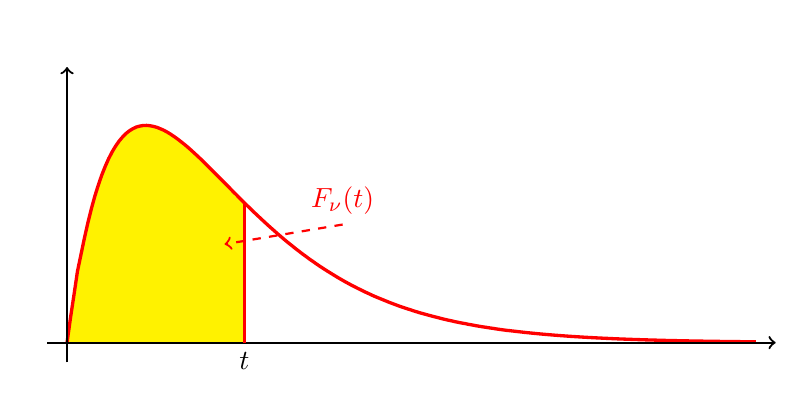
\begin{tikzpicture}[domain=0.001:17.5, samples=200, thick, scale=0.5]
		\clip (-1,-1) rectangle (18,8);
		
		\def\k{4}
		\def\g{1}
		\def\val{4.505}
		\def\fval{0.1184}
		

		\draw[fill=yellow, yscale=30, draw=none] plot[domain=0.001:\val] (\x, {exp(ln(\x/2)*\k/2 - ln(\x) - \x/2 - ln(\g))}) -- (\val, 0) -- (0.001, 0) -- cycle;
		
		\draw[very thick, color=red, yscale=30] plot (\x, {exp(ln(\x/2)*\k/2 - ln(\x) - \x/2 - ln(\g))});
		
		\draw[->] (-0.5,0) -- (18,0);
		\draw[->] (0,-0.5) -- (0,7);
		
		\draw[dashed, red, ->] (7,3) -- (4,2.5) node[at start, above, red] {$F_{\nu}(t)$};
		\draw[red] (\val, 0) -- (\val, \fval*30); % Multiplier par l'échelle y pour obtenir la bonne hauteur
		
		\node[below] at (\val, 0) {$t$};
	\end{tikzpicture}


\begin{small}
\begin{longtable}[c]{rrrrrrrrrrrrrr}
&\multicolumn{12}{c}{$p$}\\\cline{2-13}
\multicolumn{1}{c}{$\nu$} & \multicolumn{1}{c}{ $0.005$ } & \multicolumn{1}{c}{ $0.01$ } & \multicolumn{1}{c}{ $0.025$ } & \multicolumn{1}{c}{ $0.05$ } & \multicolumn{1}{c}{ $0.1$ } & \multicolumn{1}{c}{ $0.5$ } & \multicolumn{1}{c}{ $0.9$ } & \multicolumn{1}{c}{ $0.95$ } & \multicolumn{1}{c}{ $0.975$ } & \multicolumn{1}{c}{ $0.99$ } & \multicolumn{1}{c}{ $0.995$ } & \multicolumn{1}{c}{ $0.999$ }\\\midrule\endfirsthead
\multicolumn{1}{c}{$\nu$} & \multicolumn{1}{c}{ $0.005$ } & \multicolumn{1}{c}{ $0.01$ } & \multicolumn{1}{c}{ $0.025$ } & \multicolumn{1}{c}{ $0.05$ } & \multicolumn{1}{c}{ $0.1$ } & \multicolumn{1}{c}{ $0.5$ } & \multicolumn{1}{c}{ $0.9$ } & \multicolumn{1}{c}{ $0.95$ } & \multicolumn{1}{c}{ $0.975$ } & \multicolumn{1}{c}{ $0.99$ } & \multicolumn{1}{c}{ $0.995$ } & \multicolumn{1}{c}{ $0.999$ }\\\midrule\endhead
&&&&&&&&&&&&\multicolumn{1}{r}{$\rightarrow$}\endfoot
\midrule\endlastfoot

 $1$ & $0.0000$ & $0.0002$ & $0.0010$ & $0.0039$ & $0.0158$ & $0.4549$ & $2.7055$ & $3.8415$ & $5.0239$ & $6.6349$ & $7.8794$ & $10.828$ \\ 
 $2$ & $0.0100$ & $0.0201$ & $0.0506$ & $0.1026$ & $0.2107$ & $1.3863$ & $4.6052$ & $5.9915$ & $7.3778$ & $9.2103$ & $10.597$ & $13.816$ \\ 
 $3$ & $0.0717$ & $0.1148$ & $0.2158$ & $0.3518$ & $0.5844$ & $2.3660$ & $6.2514$ & $7.8147$ & $9.3484$ & $11.345$ & $12.838$ & $16.266$ \\ 
 $4$ & $0.2070$ & $0.2971$ & $0.4844$ & $0.7107$ & $1.0636$ & $3.3567$ & $7.7794$ & $9.4877$ & $11.143$ & $13.277$ & $14.860$ & $18.467$ \\ 
 $5$ & $0.4117$ & $0.5543$ & $0.8312$ & $1.1455$ & $1.6103$ & $4.3515$ & $9.2364$ & $11.070$ & $12.833$ & $15.086$ & $16.750$ & $20.515$ \\ 
 $6$ & $0.6757$ & $0.8721$ & $1.2373$ & $1.6354$ & $2.2041$ & $5.3481$ & $10.645$ & $12.592$ & $14.449$ & $16.812$ & $18.548$ & $22.458$ \\ 
 $7$ & $0.9893$ & $1.2390$ & $1.6899$ & $2.1673$ & $2.8331$ & $6.3458$ & $12.017$ & $14.067$ & $16.013$ & $18.475$ & $20.278$ & $24.322$ \\ 
 $8$ & $1.3444$ & $1.6465$ & $2.1797$ & $2.7326$ & $3.4895$ & $7.3441$ & $13.362$ & $15.507$ & $17.535$ & $20.090$ & $21.955$ & $26.124$ \\ 
 $9$ & $1.7349$ & $2.0879$ & $2.7004$ & $3.3251$ & $4.1682$ & $8.3428$ & $14.684$ & $16.919$ & $19.023$ & $21.666$ & $23.589$ & $27.877$ \\[4pt] 
 $10$ & $2.1559$ & $2.5582$ & $3.2470$ & $3.9403$ & $4.8652$ & $9.3418$ & $15.987$ & $18.307$ & $20.483$ & $23.209$ & $25.188$ & $29.588$ \\ 
 $11$ & $2.6032$ & $3.0535$ & $3.8157$ & $4.5748$ & $5.5778$ & $10.341$ & $17.275$ & $19.675$ & $21.920$ & $24.725$ & $26.757$ & $31.264$ \\ 
 $12$ & $3.0738$ & $3.5706$ & $4.4038$ & $5.2260$ & $6.3038$ & $11.340$ & $18.549$ & $21.026$ & $23.337$ & $26.217$ & $28.300$ & $32.909$ \\ 
 $13$ & $3.5650$ & $4.1069$ & $5.0088$ & $5.8919$ & $7.0415$ & $12.340$ & $19.812$ & $22.362$ & $24.736$ & $27.688$ & $29.819$ & $34.528$ \\ 
 $14$ & $4.0747$ & $4.6604$ & $5.6287$ & $6.5706$ & $7.7895$ & $13.339$ & $21.064$ & $23.685$ & $26.119$ & $29.141$ & $31.319$ & $36.123$ \\ 
 $15$ & $4.6009$ & $5.2293$ & $6.2621$ & $7.2609$ & $8.5468$ & $14.339$ & $22.307$ & $24.996$ & $27.488$ & $30.578$ & $32.801$ & $37.697$ \\ 
 $16$ & $5.1422$ & $5.8122$ & $6.9077$ & $7.9616$ & $9.3122$ & $15.338$ & $23.542$ & $26.296$ & $28.845$ & $32.000$ & $34.267$ & $39.252$ \\ 
 $17$ & $5.6972$ & $6.4078$ & $7.5642$ & $8.6718$ & $10.085$ & $16.338$ & $24.769$ & $27.587$ & $30.191$ & $33.409$ & $35.718$ & $40.790$ \\ 
 $18$ & $6.2648$ & $7.0149$ & $8.2307$ & $9.3905$ & $10.865$ & $17.338$ & $25.989$ & $28.869$ & $31.526$ & $34.805$ & $37.156$ & $42.312$ \\ 
 $19$ & $6.8440$ & $7.6327$ & $8.9065$ & $10.117$ & $11.651$ & $18.338$ & $27.204$ & $30.144$ & $32.852$ & $36.191$ & $38.582$ & $43.820$ \\[4pt] 
 $20$ & $7.4338$ & $8.2604$ & $9.5908$ & $10.851$ & $12.443$ & $19.337$ & $28.412$ & $31.410$ & $34.170$ & $37.566$ & $39.997$ & $45.315$ \\ 
 $21$ & $8.0337$ & $8.8972$ & $10.283$ & $11.591$ & $13.240$ & $20.337$ & $29.615$ & $32.671$ & $35.479$ & $38.932$ & $41.401$ & $46.797$ \\ 
 $22$ & $8.6427$ & $9.5425$ & $10.982$ & $12.338$ & $14.041$ & $21.337$ & $30.813$ & $33.924$ & $36.781$ & $40.289$ & $42.796$ & $48.268$ \\ 
 $23$ & $9.2604$ & $10.196$ & $11.689$ & $13.091$ & $14.848$ & $22.337$ & $32.007$ & $35.172$ & $38.076$ & $41.638$ & $44.181$ & $49.728$ \\ 
 $24$ & $9.8862$ & $10.856$ & $12.401$ & $13.848$ & $15.659$ & $23.337$ & $33.196$ & $36.415$ & $39.364$ & $42.980$ & $45.559$ & $51.179$ \\ 
 $25$ & $10.520$ & $11.524$ & $13.120$ & $14.611$ & $16.473$ & $24.337$ & $34.382$ & $37.652$ & $40.646$ & $44.314$ & $46.928$ & $52.620$ \\ 
 $26$ & $11.160$ & $12.198$ & $13.844$ & $15.379$ & $17.292$ & $25.336$ & $35.563$ & $38.885$ & $41.923$ & $45.642$ & $48.290$ & $54.052$ \\ 
 $27$ & $11.808$ & $12.879$ & $14.573$ & $16.151$ & $18.114$ & $26.336$ & $36.741$ & $40.113$ & $43.195$ & $46.963$ & $49.645$ & $55.476$ \\ 
 $28$ & $12.461$ & $13.565$ & $15.308$ & $16.928$ & $18.939$ & $27.336$ & $37.916$ & $41.337$ & $44.461$ & $48.278$ & $50.993$ & $56.892$ \\ 
 $29$ & $13.121$ & $14.256$ & $16.047$ & $17.708$ & $19.768$ & $28.336$ & $39.087$ & $42.557$ & $45.722$ & $49.588$ & $52.336$ & $58.301$ \\
 $30$ & $13.787$ & $14.953$ & $16.791$ & $18.493$ & $20.599$ & $29.336$ & $40.256$ & $43.773$ & $46.979$ & $50.892$ & $53.672$ & $59.703$ \\ 
\end{longtable}
\end{small}
\end{center}

\section{Loi de Student}
$$F_{\nu}(t)=\prob(X \leq t)$$

La table suivante contient les quantiles de la loi de Student avec $\nu$ degrés de liberté. Pour tout $0<p<1$, le quantile est la valeur de $t$ pour laquelle $\prob\{X\leq t\}=p$, où $X\sim St(\nu)$. Ainsi $t=F^{-1}_{\nu}(p)$.


Cette table ne contient que les quantiles pour des valeurs $p\geq \frac{1}{2}$. Si $p<\frac{1}{2}$, les quantiles peuvent être obtenus par symétrie de la loi : $F_{\nu}^{-1}(p)=-F_{\nu}^{-1}(1-p)$.

\begin{center}

\begin{tikzpicture}[
	declare function={gamma(\z)=2.506628274631*sqrt(1/\z) + 0.20888568*(1/\z)^(1.5) + 0.00870357*(1/\z)^(2.5) - (174.2106599*(1/\z)^(3.5))/25920 - (715.6423511*(1/\z)^(4.5))/1244160)*exp((-ln(1/\z)-1)*\z;},
	declare function={student(\x,\n)=gamma((\n+1)/2)/(sqrt(\n*pi)*gamma(\n/2))*(1+(\x*\x)/\n)^(-(\n+1)/2);}
	]
	\begin{axis}[
		domain=-5:5, samples=100,
		axis lines=middle,
		enlarge x limits=false,
		enlarge y limits=true,
		ytick=\empty,
		xtick=\empty,
		no markers,
		x label style={at={(axis description cs:1.05,0.5)},anchor=south},
		y label style={at={(axis description cs:0.5,1.05)},anchor=west}
		]
		\def\n{4}
		\def\val{-0.7}
		\def\fval{0.282}
		\addplot+[very thick,red,name path=A] {student(x,\n)};
		\addplot+[draw=none,name path=B] {0};
		\addplot+[yellow] fill between[of=A and B,soft clip={domain=-4:\val}];
		\draw[dashed,red,->] (axis cs: -3,0.2) -- (axis cs: -1.5,0.05) node[at start,above] {$F_{\nu}(t)$};
		\draw[red] (axis cs: \val,0) -- (axis cs: \val,\fval);
		\node[below] at (axis cs: \val,0) {$t$};
	\end{axis}
\end{tikzpicture}

\begin{small}
\begin{longtable}[c]{rrrrrrrrrrrrrr}
&\multicolumn{12}{c}{$p$}\\\cline{2-13}
\multicolumn{1}{c}{$\nu$} & \multicolumn{1}{c}{ $0.6$ } & \multicolumn{1}{c}{ $0.7$ } & \multicolumn{1}{c}{ $0.75$ } & \multicolumn{1}{c}{ $0.8$ } & \multicolumn{1}{c}{ $0.85$ } & \multicolumn{1}{c}{ $0.9$ } & \multicolumn{1}{c}{ $0.95$ } & \multicolumn{1}{c}{ $0.975$ } & \multicolumn{1}{c}{ $0.99$ } & \multicolumn{1}{c}{ $0.995$ } & \multicolumn{1}{c}{ $0.999$ } & \multicolumn{1}{c}{ $0.9995$ }\\\midrule\endfirsthead
\multicolumn{1}{c}{$\nu$} & \multicolumn{1}{c}{ $0.6$ } & \multicolumn{1}{c}{ $0.7$ } & \multicolumn{1}{c}{ $0.75$ } & \multicolumn{1}{c}{ $0.8$ } & \multicolumn{1}{c}{ $0.85$ } & \multicolumn{1}{c}{ $0.9$ } & \multicolumn{1}{c}{ $0.95$ } & \multicolumn{1}{c}{ $0.975$ } & \multicolumn{1}{c}{ $0.99$ } & \multicolumn{1}{c}{ $0.995$ } & \multicolumn{1}{c}{ $0.999$ } & \multicolumn{1}{c}{ $0.9995$ }\\\midrule\endhead
&&&&&&&&&&&&\multicolumn{1}{r}{$\rightarrow$}\endfoot
\midrule\endlastfoot

 $1$ & $0.3249$ & $0.7265$ & $1.0000$ & $1.3764$ & $1.9626$ & $3.0777$ & $6.3138$ & $12.706$ & $31.821$ & $63.657$ & $318.31$ & $636.62$ \\ 
 $2$ & $0.2887$ & $0.6172$ & $0.8165$ & $1.0607$ & $1.3862$ & $1.8856$ & $2.9200$ & $4.3027$ & $6.9646$ & $9.9248$ & $22.327$ & $31.599$ \\ 
 $3$ & $0.2767$ & $0.5844$ & $0.7649$ & $0.9785$ & $1.2498$ & $1.6377$ & $2.3534$ & $3.1824$ & $4.5407$ & $5.8409$ & $10.215$ & $12.924$ \\ 
 $4$ & $0.2707$ & $0.5686$ & $0.7407$ & $0.9410$ & $1.1896$ & $1.5332$ & $2.1318$ & $2.7764$ & $3.7469$ & $4.6041$ & $7.1732$ & $8.6103$ \\ 
 $5$ & $0.2672$ & $0.5594$ & $0.7267$ & $0.9195$ & $1.1558$ & $1.4759$ & $2.0150$ & $2.5706$ & $3.3649$ & $4.0321$ & $5.8934$ & $6.8688$ \\ 
 $6$ & $0.2648$ & $0.5534$ & $0.7176$ & $0.9057$ & $1.1342$ & $1.4398$ & $1.9432$ & $2.4469$ & $3.1427$ & $3.7074$ & $5.2076$ & $5.9588$ \\ 
 $7$ & $0.2632$ & $0.5491$ & $0.7111$ & $0.8960$ & $1.1192$ & $1.4149$ & $1.8946$ & $2.3646$ & $2.9980$ & $3.4995$ & $4.7853$ & $5.4079$ \\ 
 $8$ & $0.2619$ & $0.5459$ & $0.7064$ & $0.8889$ & $1.1081$ & $1.3968$ & $1.8595$ & $2.3060$ & $2.8965$ & $3.3554$ & $4.5008$ & $5.0413$ \\ 
 $9$ & $0.2610$ & $0.5435$ & $0.7027$ & $0.8834$ & $1.0997$ & $1.3830$ & $1.8331$ & $2.2622$ & $2.8214$ & $3.2498$ & $4.2968$ & $4.7809$ \\[4pt] 
 $10$ & $0.2602$ & $0.5415$ & $0.6998$ & $0.8791$ & $1.0931$ & $1.3722$ & $1.8125$ & $2.2281$ & $2.7638$ & $3.1693$ & $4.1437$ & $4.5869$ \\ 
 $11$ & $0.2596$ & $0.5399$ & $0.6974$ & $0.8755$ & $1.0877$ & $1.3634$ & $1.7959$ & $2.2010$ & $2.7181$ & $3.1058$ & $4.0247$ & $4.4370$ \\ 
 $12$ & $0.2590$ & $0.5386$ & $0.6955$ & $0.8726$ & $1.0832$ & $1.3562$ & $1.7823$ & $2.1788$ & $2.6810$ & $3.0545$ & $3.9296$ & $4.3178$ \\ 
 $13$ & $0.2586$ & $0.5375$ & $0.6938$ & $0.8702$ & $1.0795$ & $1.3502$ & $1.7709$ & $2.1604$ & $2.6503$ & $3.0123$ & $3.8520$ & $4.2208$ \\ 
 $14$ & $0.2582$ & $0.5366$ & $0.6924$ & $0.8681$ & $1.0763$ & $1.3450$ & $1.7613$ & $2.1448$ & $2.6245$ & $2.9768$ & $3.7874$ & $4.1405$ \\ 
 $15$ & $0.2579$ & $0.5357$ & $0.6912$ & $0.8662$ & $1.0735$ & $1.3406$ & $1.7531$ & $2.1314$ & $2.6025$ & $2.9467$ & $3.7328$ & $4.0728$ \\ 
 $16$ & $0.2576$ & $0.5350$ & $0.6901$ & $0.8647$ & $1.0711$ & $1.3368$ & $1.7459$ & $2.1199$ & $2.5835$ & $2.9208$ & $3.6862$ & $4.0150$ \\ 
 $17$ & $0.2573$ & $0.5344$ & $0.6892$ & $0.8633$ & $1.0690$ & $1.3334$ & $1.7396$ & $2.1098$ & $2.5669$ & $2.8982$ & $3.6458$ & $3.9651$ \\ 
 $18$ & $0.2571$ & $0.5338$ & $0.6884$ & $0.8620$ & $1.0672$ & $1.3304$ & $1.7341$ & $2.1009$ & $2.5524$ & $2.8784$ & $3.6105$ & $3.9216$ \\ 
 $19$ & $0.2569$ & $0.5333$ & $0.6876$ & $0.8610$ & $1.0655$ & $1.3277$ & $1.7291$ & $2.0930$ & $2.5395$ & $2.8609$ & $3.5794$ & $3.8834$ \\[4pt] 
 $20$ & $0.2567$ & $0.5329$ & $0.6870$ & $0.8600$ & $1.0640$ & $1.3253$ & $1.7247$ & $2.0860$ & $2.5280$ & $2.8453$ & $3.5518$ & $3.8495$ \\ 
 $21$ & $0.2566$ & $0.5325$ & $0.6864$ & $0.8591$ & $1.0627$ & $1.3232$ & $1.7207$ & $2.0796$ & $2.5176$ & $2.8314$ & $3.5272$ & $3.8193$ \\ 
 $22$ & $0.2564$ & $0.5321$ & $0.6858$ & $0.8583$ & $1.0614$ & $1.3212$ & $1.7171$ & $2.0739$ & $2.5083$ & $2.8188$ & $3.5050$ & $3.7921$ \\ 
 $23$ & $0.2563$ & $0.5317$ & $0.6853$ & $0.8575$ & $1.0603$ & $1.3195$ & $1.7139$ & $2.0687$ & $2.4999$ & $2.8073$ & $3.4850$ & $3.7676$ \\ 
 $24$ & $0.2562$ & $0.5314$ & $0.6848$ & $0.8569$ & $1.0593$ & $1.3178$ & $1.7109$ & $2.0639$ & $2.4922$ & $2.7969$ & $3.4668$ & $3.7454$ \\ 
 $25$ & $0.2561$ & $0.5312$ & $0.6844$ & $0.8562$ & $1.0584$ & $1.3163$ & $1.7081$ & $2.0595$ & $2.4851$ & $2.7874$ & $3.4502$ & $3.7251$ \\ 
 $26$ & $0.2560$ & $0.5309$ & $0.6840$ & $0.8557$ & $1.0575$ & $1.3150$ & $1.7056$ & $2.0555$ & $2.4786$ & $2.7787$ & $3.4350$ & $3.7066$ \\ 
 $27$ & $0.2559$ & $0.5306$ & $0.6837$ & $0.8551$ & $1.0567$ & $1.3137$ & $1.7033$ & $2.0518$ & $2.4727$ & $2.7707$ & $3.4210$ & $3.6896$ \\ 
 $28$ & $0.2558$ & $0.5304$ & $0.6834$ & $0.8546$ & $1.0560$ & $1.3125$ & $1.7011$ & $2.0484$ & $2.4671$ & $2.7633$ & $3.4082$ & $3.6739$ \\ 
 $29$ & $0.2557$ & $0.5302$ & $0.6830$ & $0.8542$ & $1.0553$ & $1.3114$ & $1.6991$ & $2.0452$ & $2.4620$ & $2.7564$ & $3.3962$ & $3.6594$ \\
 $30$ & $0.2556$ & $0.5300$ & $0.6828$ & $0.8538$ & $1.0547$ & $1.3104$ & $1.6973$ & $2.0423$ & $2.4573$ & $2.7500$ & $3.3852$ & $3.6460$ \\ 
\end{longtable}
\end{small}           \end{center}